\documentclass[11pt]{article}
\usepackage[a4paper, total={6in, 8in}]{geometry}
\usepackage[export]{adjustbox}
\usepackage[utf8]{inputenc}
\usepackage{hyperref}
\usepackage{graphics}
\usepackage{amssymb}

\hypersetup{
    colorlinks=false
}
\urlstyle{same}
\graphicspath{ {./images/} }
\everymath{\displaystyle}

\title
{%
  {\Huge CS412 Final Project \\
  \Huge Travelling Salesman Problem\\
    \huge Implementations and Analysis of Various Solutions}
}
\date{\Large \today}
\begin{document}
\maketitle
\centering
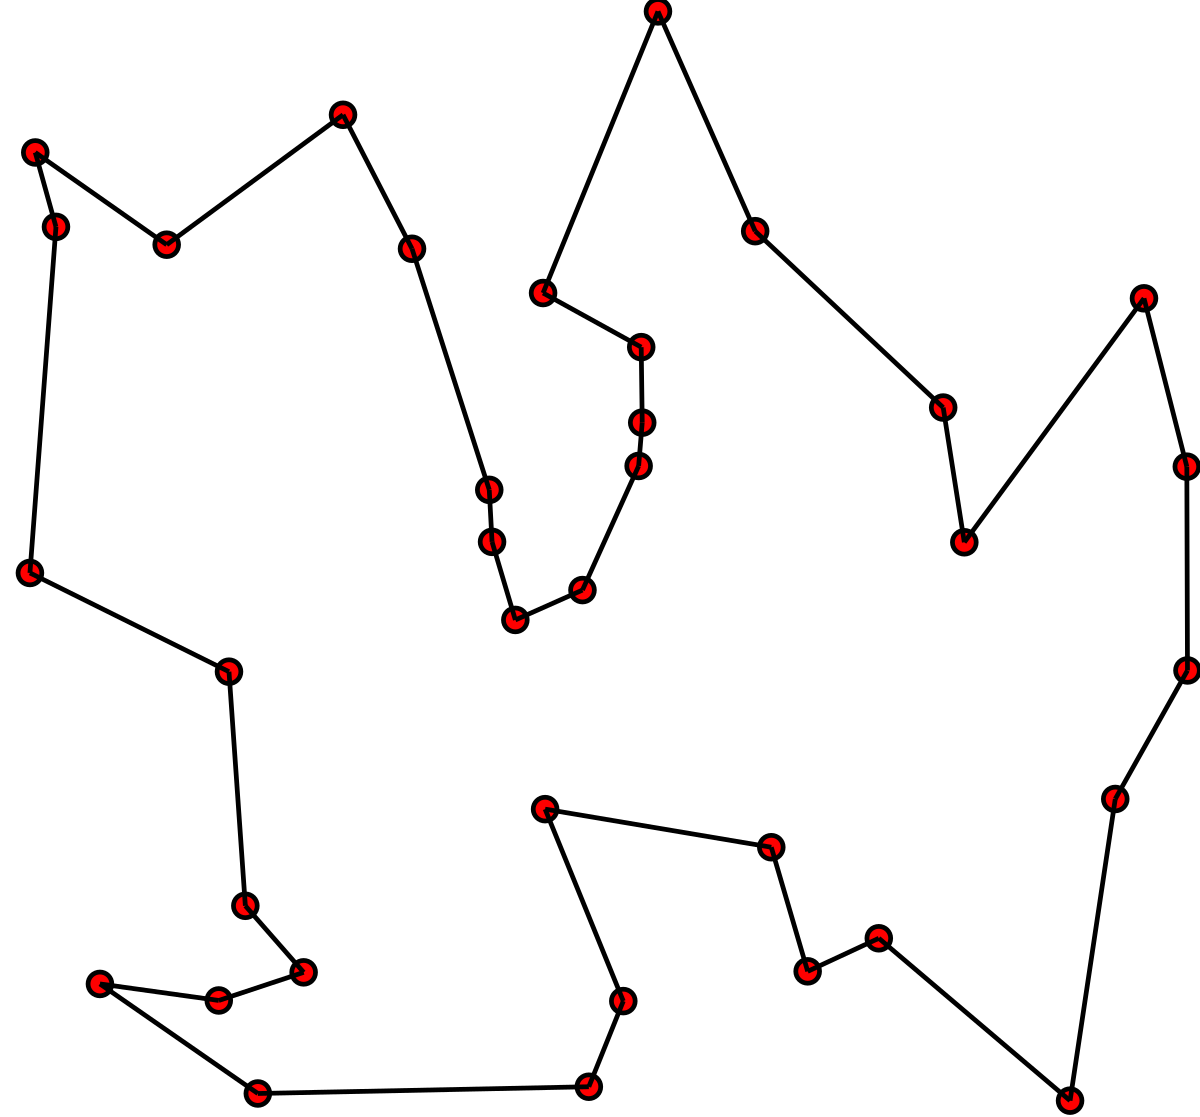
\includegraphics[scale=0.2]{images/title.png}
\newpage
\paragraph{}
\paragraph{}
\paragraph{}
\paragraph{}
\paragraph{}
\paragraph{}
\paragraph{}
\paragraph{}
\paragraph{}
\par \centering
This page is has been intentionally left blank intentionally \paragraph{}
The typo in the sentence above is left unfixed intentionally as well, because leaving a page intentionally blank makes the same amount of sense as leaving a typo in a sentence intentionally unfixed. 
\par \flushleft

\newpage
\tableofcontents

\newpage


\newpage
\section{Introduction}
The travelling salesman problem has a long history of being a problem of interest in the field of algorithms. It has garnered much attention and there has been a lot of work that has been done on it. In this project we will set out to establish the details of this problem and why it is so tough. We will then investigate 4 algorithms that have become well known in being useful for solving this problem. One of them produces an exact solution and the rest use approximation techniques. We will be using theory and implementation to test the runtimes of this problem and will then present our research in an appropriate format.
\section{Design Techniques}
	\subsection{Exact Solution}
		\subsubsection{ Held-Karp Algorithm}
		
	\subsection{ Approximate Solutions}
		\subsubsection {Nearest Neighbour Algorithm}
		\subsubsection {Pairwise Exchange Method}
		\subsubsection {Christofides–Serdyukov Algorithm}
		
\section{Theoretical Runtime Analysis and Comparison}
\section{Empirical Runtime Analysis and Comparison}
\section{Conclusion}
\newpage
\section{References}
\begin{enumerate}
	\item \url{https://www.researchgate.net/publication/289195926_On_the_Nearest_Neighbor_Algorithms_for_the_Traveling_Salesman_Problem}
	\item \url{https://en.wikipedia.org/wiki/Travelling_salesman_problem#:~:text=The%20travelling%20salesman%20problem%20}
	\item Thomas H. Cormen, Charles E. Leiserson, Ronald L. Rivest, and Clifford Stein. 2009. Introduction to Algorithms, Third Edition (3rd. ed.)
	\item David L. Applegate, Robert E. Bixby, Vasek Chvatal, and William J. Cook. 2007. The Traveling Salesman Problem: A Computational Study. Princeton University Press, USA.
\end{enumerate}




\end{document}